\begin{figure}[h]
    \centering
    \captionsetup{width=.9\linewidth}
    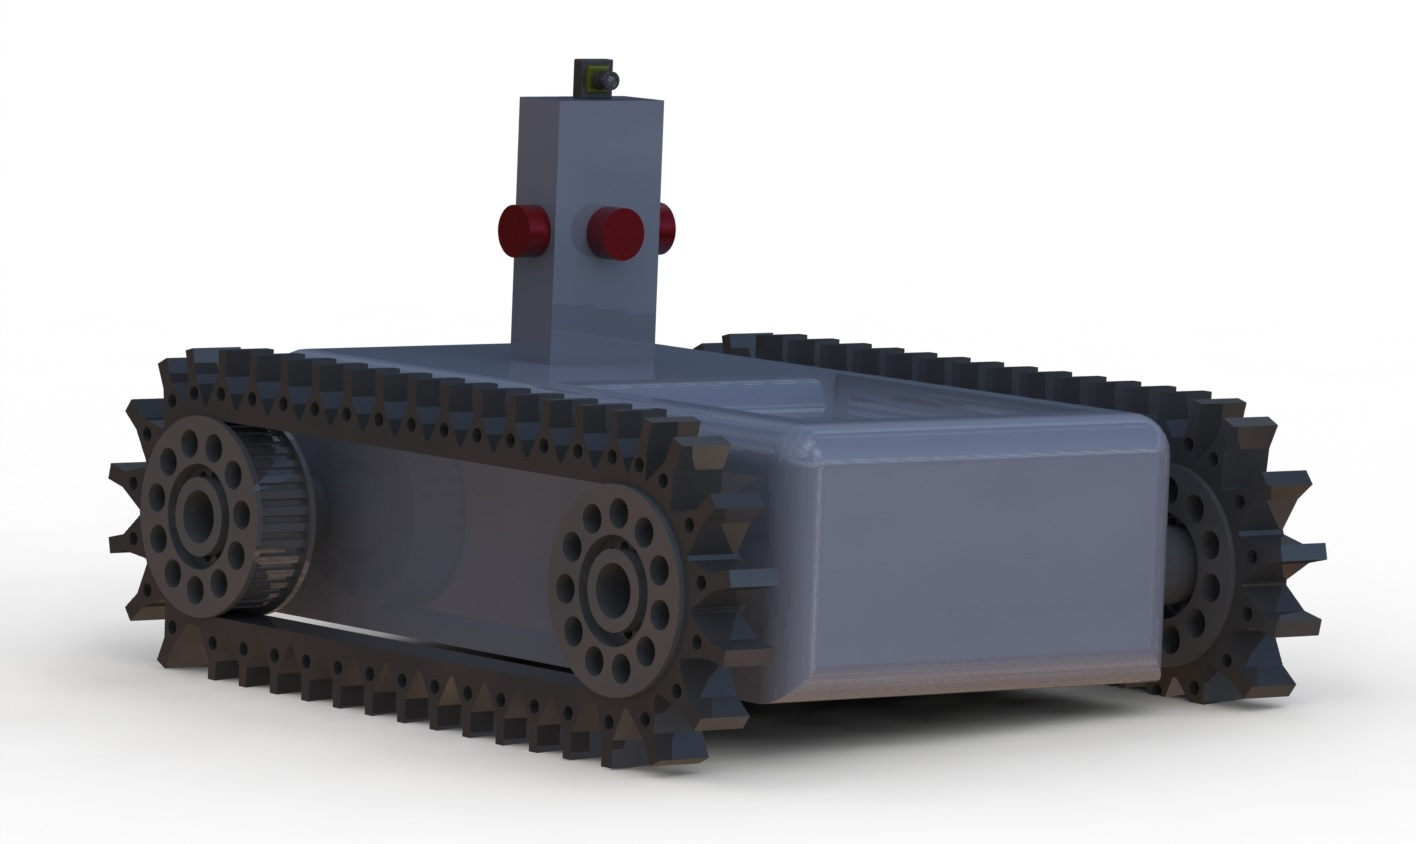
\includegraphics[width=1\linewidth]{v2_rendering.JPG}
    \caption{Erster Prototyp}
    \label{fig:prot}
\end{figure}

Das 3D-Modell des Rettungsroboters wurde mit der Software SolidWorks erstellt. Die Abbildung \ref{fig:prot} zeigt den ersten Prototyp. Hier wurden schon der Kettenantrieb und eine Ablagefläche für ein Erste-Hilfe-Kit umgesetzt. Weiter wurde auf dem Robotor ein Turm platziert, um dort 4 Sensroen für die Orientierung anzubringen. Oben auf dem Turm befindet sich eine Kamera.\\


\begin{figure}[h]
    \centering
    \captionsetup{width=.9\linewidth}
    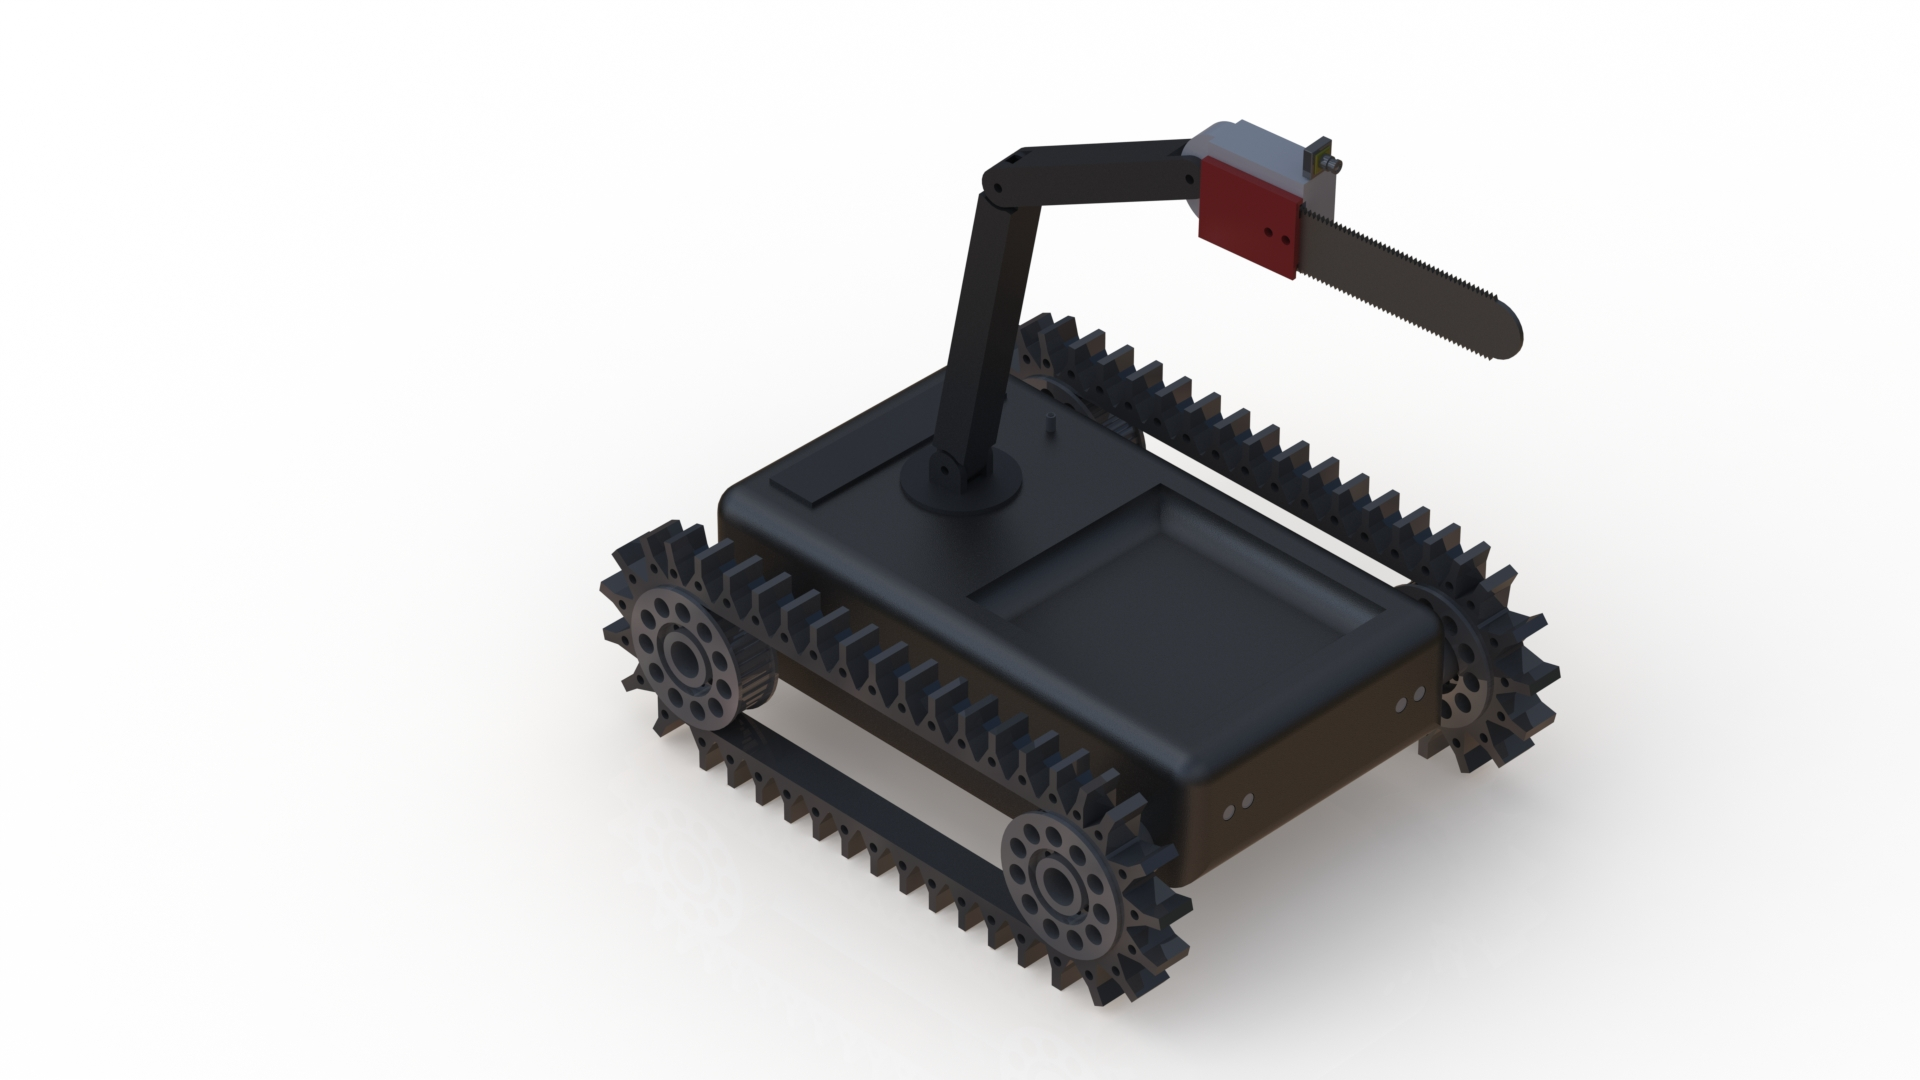
\includegraphics[width=1\linewidth]{bot_rendering_v4.JPG}
    \caption{Zweite Version des Roboters}
    \label{fig:second}
\end{figure}

Für die zweite Version des Prototyps wurde zunächst der Körper des Bots angepasst. Für eine Verbesserung des Strömungsverhaltens und einer Erhöhung des Böschungswinkels wurde der Körper an der vorderen unteren Kante mit einer sehr flachen Fase versehen.

Im nächsten Schritt wurde der unbewegliche Turm durch einen Roboterarm mit 3 Gelenken und einer Drehscheibe ersetzt (Abb. \ref{fig:second}). Am Ende des Arms wurde eine Kettensäge angebracht. Die Kamera wurde auf der Säge angebracht, um so die Säge immer im Blick zu haben.

Weiter wurden noch ein austauschbarer Akku, ein omnidirektionales Mikrofon und Ultraschallsensoren in den Prototyp intgeriert.\\
\begin{figure}[h]
    \centering
    \captionsetup{width=.9\linewidth}
    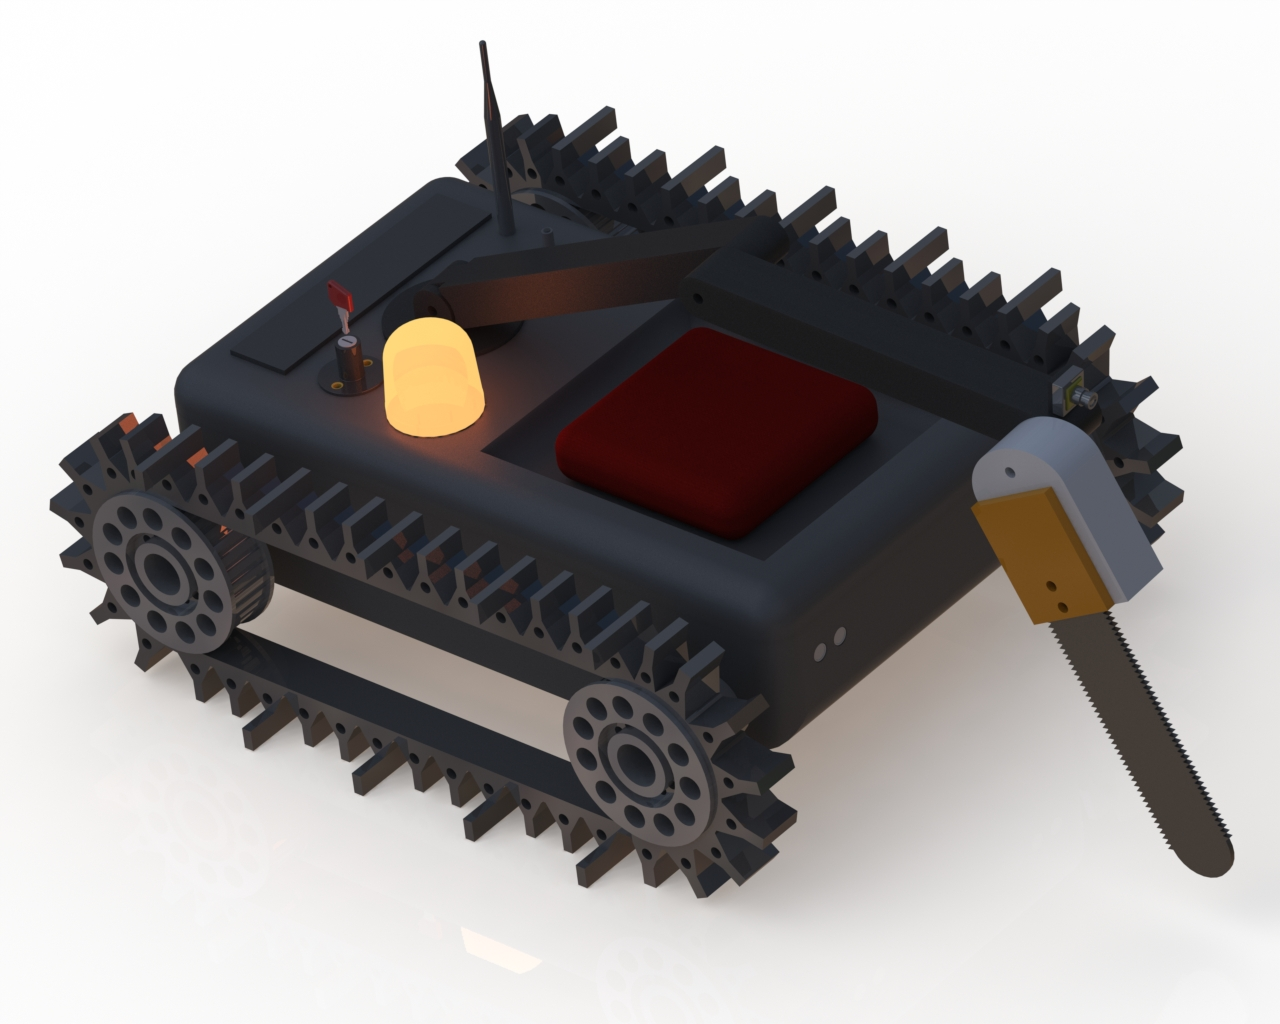
\includegraphics[width=1\linewidth]{trimetrisch_vorne_rechts_oben.JPG}
    \caption{Außenansicht des finalen Roboters}
    \label{fig:final}
\end{figure}
Abbildung \ref{fig:context} zeigt das finale Modell. Im Vergleich  zur vorherigen Version noch folgende Elemente hinzugefügt:
\begin{itemize}
    \item Rundumleuchte
    \item Antenne
    \item Ein/Aus-Schalter
    \item seitliche Paddel an den Ketten\\
\end{itemize}

Der komplette Arm des Roboters hat eine Revision erfahren, so dass die beiden Teilarme und die Säge eingeklappt werden können. Die Kamera wurde auf den oberen Arm versetzt, damit die Kettensäge eingeklappt werden kann und der Operator trotzdem die Sicht nach Vorn behält.

Außerdem wurde der Hauptkörper des Roboters in eine Wanne und einen Deckel unterteilt, um zum Einen die Teile druckbar zu machen und zum ist nur so möglich die benötigte Hardware (Motoren, Mikrocontroller, usw.) zu installieren.  \\

Die Abbildungen \ref{fig:top} und \ref{fig:front} zeigen, dass für die vorgesehene Hardware genug Platz vorhanden ist und auch entsprechende Befestigungspunkte vorhanden sind.\\
\begin{figure}[h]
    \centering
    \captionsetup{width=.9\linewidth}
    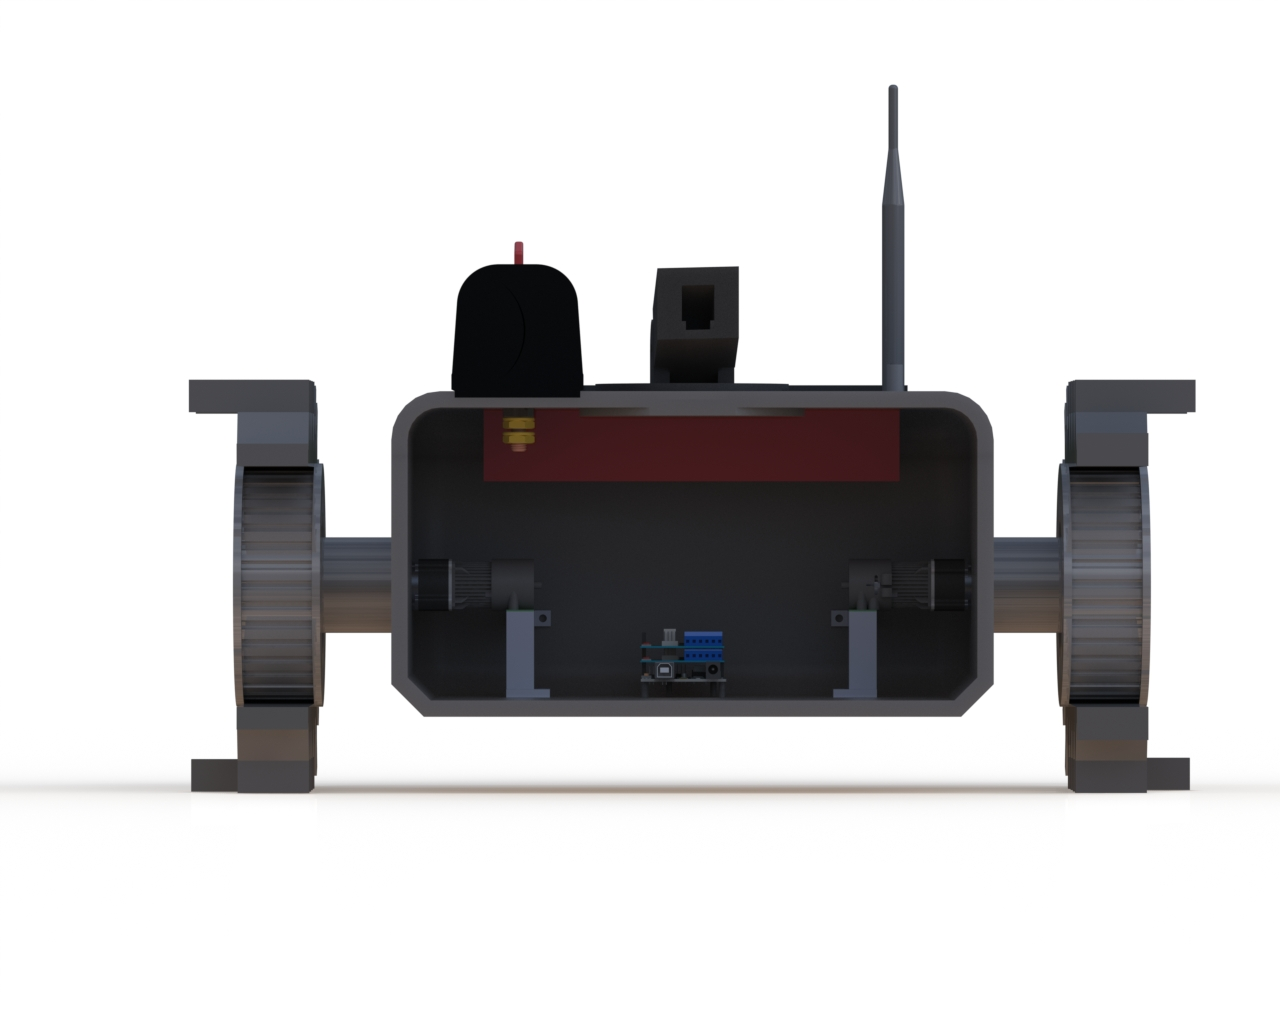
\includegraphics[width=1\linewidth]{schnitt_front.JPG}
    \caption{Schnittansicht von vorne}
    \label{fig:front}
\end{figure}\\
\begin{figure}[h]
    \centering
    \captionsetup{width=.9\linewidth}
    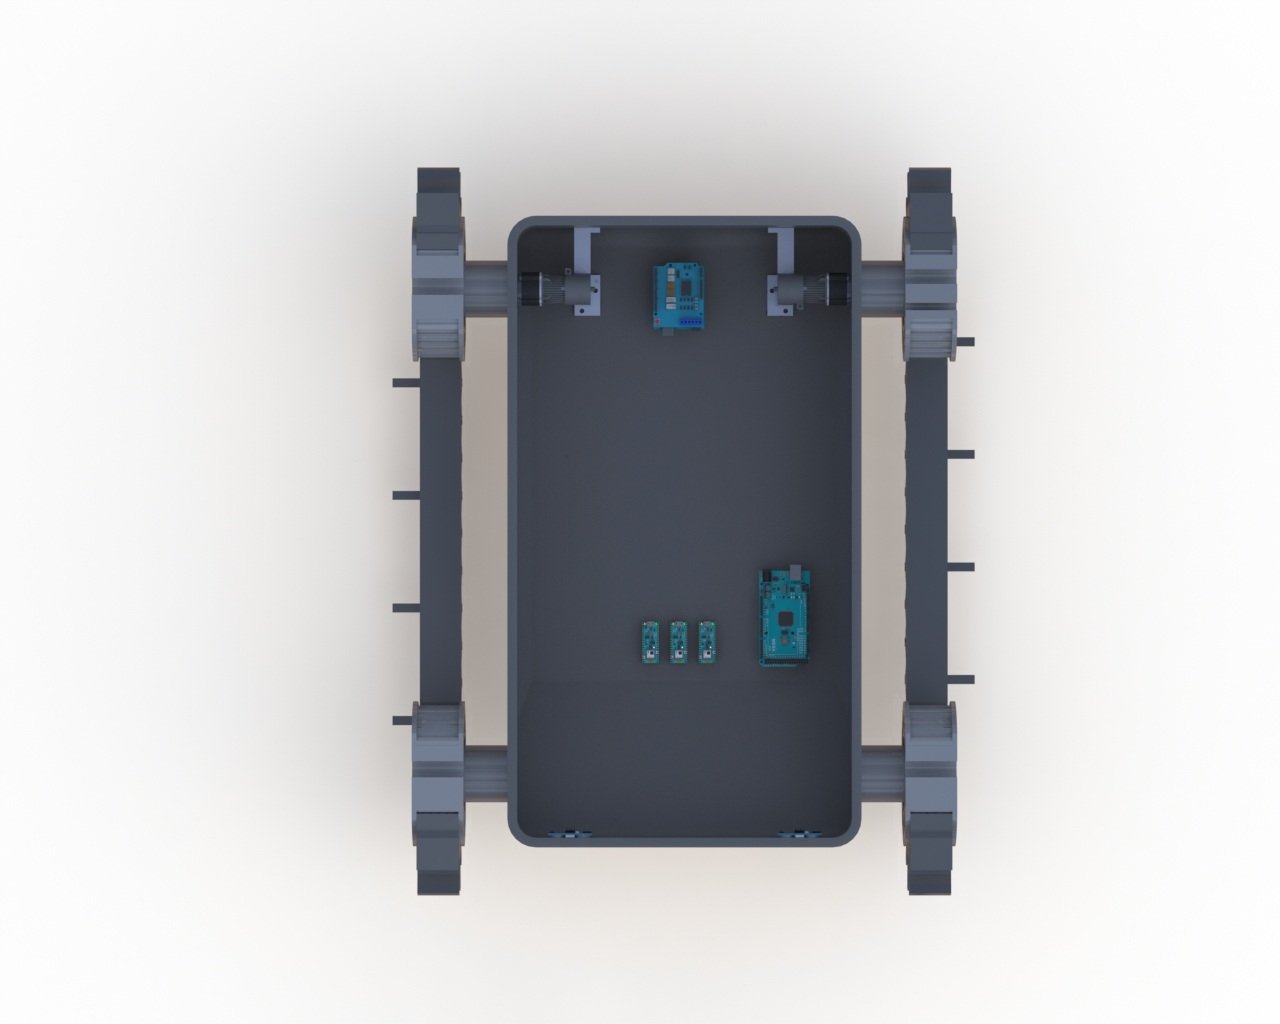
\includegraphics[width=1\linewidth]{schnitt_top.JPG}
    \caption{Schnittansicht von oben}
    \label{fig:top}
\end{figure}\\
Zum Schluss wurden alle Druckteile mit Hilfe des Felix Repetier Hosts auf Druckbarkeit überprüft. Abbildung \ref{fig:print_stats} zeigt die Statistiken für einen 3D-Druck mit 25\% Infill  und ABS Filament. Aus der benötigten Filamentmenge und der spezifischen Materialdichte lässt sich das Gewicht der Druckteile errechnen (Abb. \ref{fig:filament_weight}). Hier ergibt sich ein Gewicht von etwa 5,67 kg.

In Solidworks wurde für die Wanne des Hauptkörpers ein Volumen von etwa 7,9 Liter berechnet. Daraus lässt sich schließen, dass der Roboter ein Gesamtgewicht von 7,9 kg nicht überschreiten sollte. Da die Druckteile schon 5,67 kg  wiegen, bleiben für die restlichen Teile (Motoren, Akku, Elektronik, Säge, Lager, Erste-Hilfe-Kit) nur etwa 2,23 kg.
Das wäre nicht sinngemäß zu realisieren. Das bedeutet der Hauptkörper sollte noch deutlich vergrößert werden. Zusätzlich könnten die Wandstärken verringert werden, um Gewicht zu Sparen. Für die Teile des Roboterarms würde sich ein Fachwerk anbieten. 
\begin{figure}[h]
    \centering
    \captionsetup{width=.9\linewidth}
    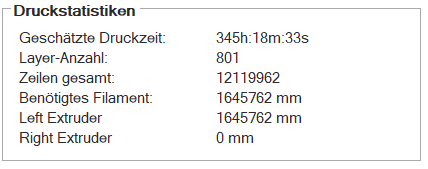
\includegraphics[width=1\linewidth]{print-statistic.PNG}
    \caption{Druckstatistiken}
    \label{fig:print_stats}
\end{figure}
\begin{figure}[h]
    \centering
    \captionsetup{width=.9\linewidth}
    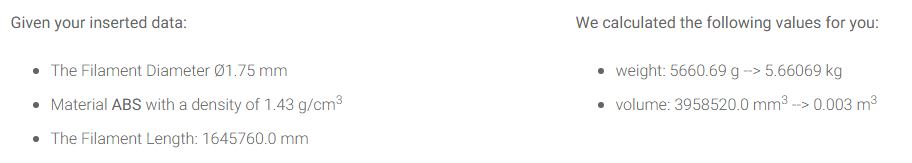
\includegraphics[width=1\linewidth]{filament_weight.PNG}
    \caption{Erechnetes Filamentgewicht}
    \label{fig:filament_weight}
\end{figure}